\chapter{Einstein's Euqation}
In this chapter we shall give a mathematically precise formulation of the ideas sketched in the introduction. We begin by giving an exposition of the elementary topic of the geometry of space and the spatial tensorial character of physical laws in prerelativity physics. The discussion of special relativity which follows will completely parallel this discussion, with ``spacetime'' replacing ``space''. Our next (and most important) task will be to formulate general relativity and provide a motivation for Einstein's equation, which relates the geometry of spacetime to the distribution of matter in the universe. Finally, we will examine general relativity in the limit where gravity is weak. We will show that in appropriate circumstances general relativity reproduces the predictions of the Newtonian theory of gravity. We aIso will show that in general relativity, gravity has dynamical degrees of freedom which can be excited by the motion of matter, i.e., that general relativity predicts the existence of gravitational radiation.

\section{The Geometry of Space in Prerelativity Physics; General and Special Covariance}
\section{Special Relativity}
\label{4.2.2}
% \begin{equation}
%     \eta_{ab}=\sum_{\mu,\nu=0}^3\eta_{\mu\nu}(\d x^\mu)_a(\d x^\nu)_b
%     \label{4.2.2}
% \end{equation}

\section{General Relativity}
\section{Linearized Gravity: The Newtonian Limit and Gravitational Radiation}

% \includepdf[pages=31-42]{document}